\chapter{}

%\begin{figure}[p]
%    \hspace*{-2.5cm}
%    \makebox[\linewidth]{
%        \setlength{\fboxsep}{0pt}
%        \fbox{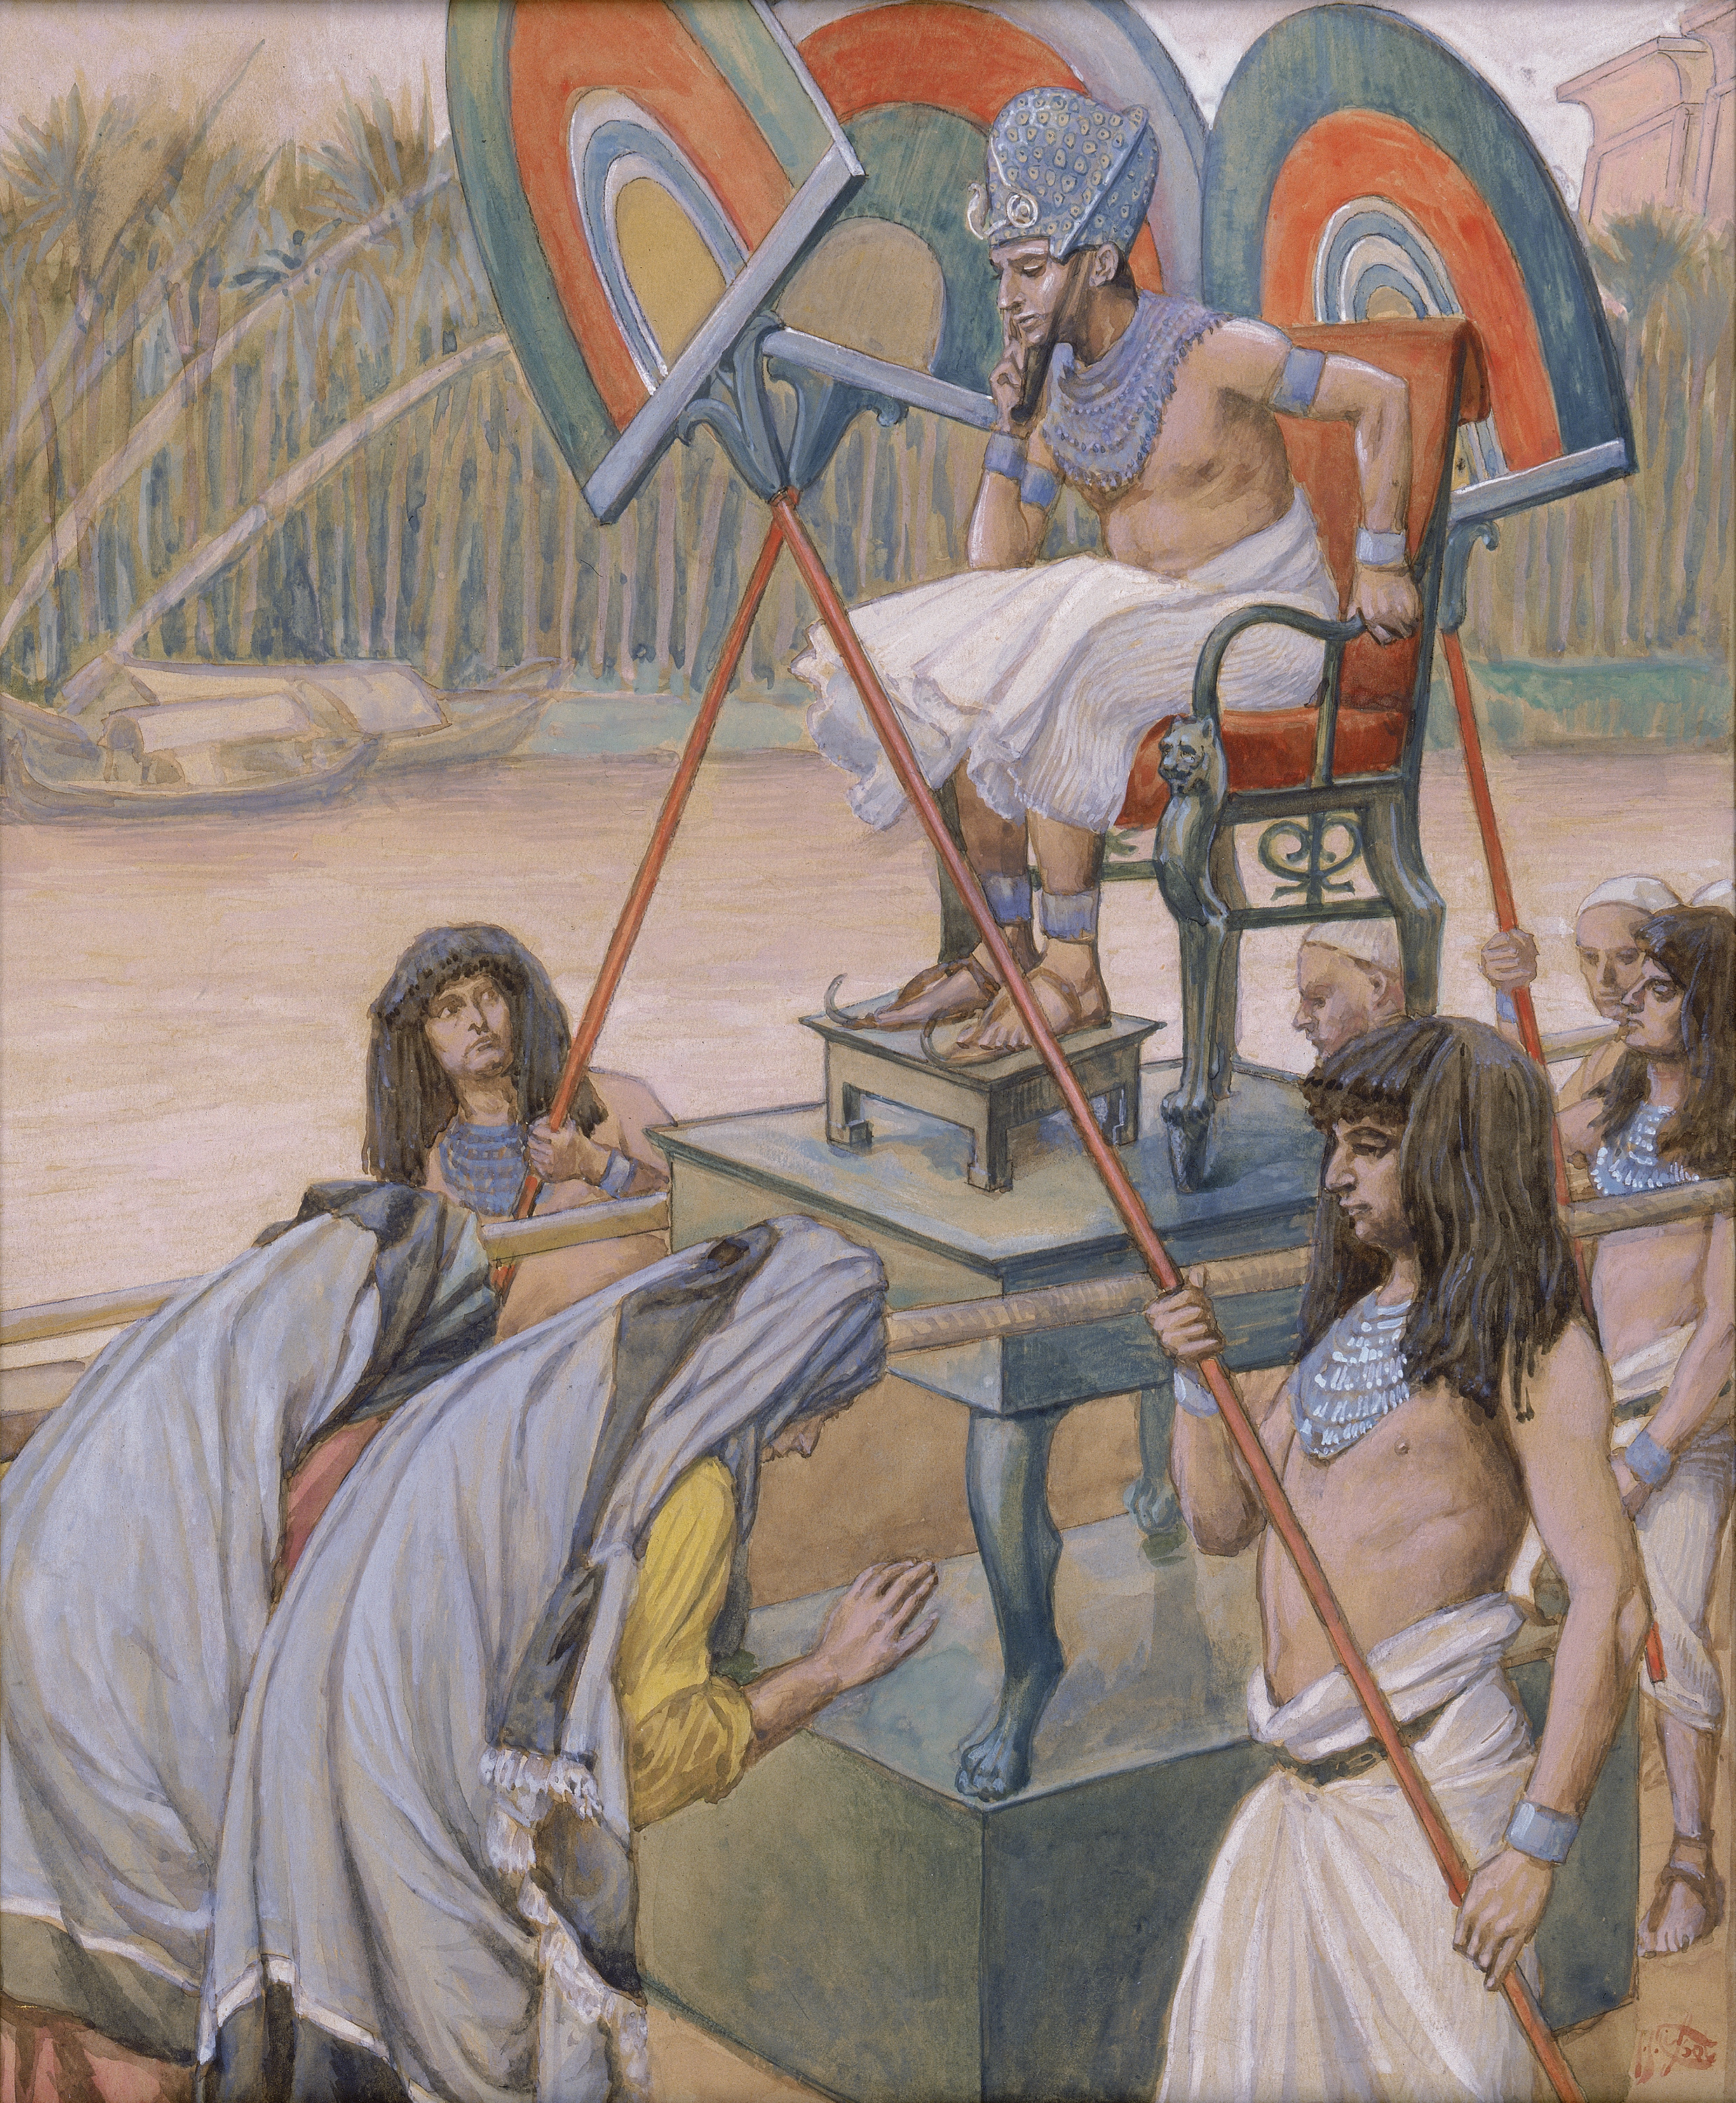
\includegraphics[width=1.3\linewidth]{midwives}}
%    }
%    \caption{\hspace*{-4.5cm}Obstetricēs et Rēx}
%\end{figure}

\titleimg{mw2.jpg}

{\begin{center}\large\bf\underline{Capitulum Primum}\end{center}%}

[In Aegyptō] fīliī Isrāēl crēvērunt, et \marginpar{quasi germinantēs: non vero germinantēs (quia hominēs non germinant) sed vidērī aliquō modō germināre}quasi\marginpar{germināre: emittere germina (ea quae ex plantīs veniunt: semen, fructus, cēt.)} germinantēs \marginpar{multiplicāre: multum facere; augēre}multiplicātī sunt:
ac rōborātī \marginpar{rōborāre: virēs dāre}nimis, implēvērunt terram.

Surrēxit intereā rēx novus super Ægyptum, quī ignōrābat Ioseph.
Et ait ad populum suum: ``Ecce, populus fīliōrum Isrāēl multus, et fortior nōbīs est.
Venīte, \marginpar{{\bf sapienter (adv) <} sapiēns}\marginpar{opprimere: efficere ut aliquis surgere nōn potest}\marginpar{ingruere: cum vi accedere}sapienter opprimāmus eum, nē forte multiplicētur: et sī ingruerit contrā nōs bellum, addātur inimīcīs nostrīs, expugnātisque nōbīs ēgrediātur dē terrā.''

\begin{figure}[h]
    \begin{minipage}[h]{0.5\linewidth}
        \centering
        
\includegraphics{tab}
        \caption{tabernaculum, -ī (n)}
    \end{minipage}%
    \begin{minipage}[h]{0.5\linewidth}
        \vspace*{-0.3cm}
        \centering
        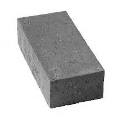
\includegraphics{later}
        \vspace*{-0.425cm}
        \caption{later, lateris (m)}
    \end{minipage}
\end{figure}

Præposuit \marginpar{praeposuit eīs magistrōs operum: dedit magistrīs potestatem super opera fīliōrum Isrāēl}itaque eīs magistrōs operum, ut afflīgerent eōs \marginpar{onus, oneris (n): res quam difficile est portare vel agere. e.g: saccus lapidibus plenus, labor difficilis} oneribus: 
ædificaveruntquē urbēs tabernāculōrum Pharaōnī, Phithom et Ramessēs.
Quantōque opprimēbant eōs, tantō magis multiplicābantur, et crēscēbant: 
ōderantque fīliōs Isrāēl Ægyptiī, et afflīgēbant \marginpar{illūdere: deridēre}illūdentēs eīs,
atque ad \marginpar{{\bf amāritūdo, -inis (f)}\\\hspace{0.5cm} < amārus/a/um $\leftrightarrow$ dulcis, -e}amāritūdinem \marginpar{per-dūcere: trahere}perdūcēbant vītam eōrum operibus dūrīs \marginpar{lutum, -ī(n): terra humida}lutī et lateris, omnīque \marginpar{famulātus, -ūs (m): servitus; conditiō servōrum}famulātū, quō in terræ operibus premēbantur. 
Dīxit autem rēx Ægyptī \marginpar{obstetrix, -īcis(f): femina quae iuvat feminam gravidam parere} obstetrīcibus Hebræōrum, quārum ūna vocābātur Sephora, altera Phua, 
\marginpar{praecipere: imperāre} præcipiēns eīs: ``Quandō obstetrīcābitis Hebræās, et \marginpar{partus, -ūs (m): actus pariendi} partus tempus advēnerit: sī masculus fuerit, interficite eum: sī fēmina, \marginpar{reservāre: servāre, conservāre}reservātē.''

Timuērunt autem obstetrīcēs Deum, \marginpar{praeceptum, -ī: quod praecipitur}\marginpar{nōn fēcērunt iuxtā praeceptum regis: non parent praeceptō rēgis}et nōn fēcērunt iuxtā præceptum rēgis Ægyptī, sed \marginpar{cōnservāre: servāre}cōnservābant \marginpar{mas, maris(m): homo (vel animal) masculinus}marēs. 
Quibus ad sē accersītis, rēx ait: ``Quidnam est hoc quod facere voluistis, ut puerōs servārētis?''

Quæ respondērunt: ``Nōn sunt Hebreæ sīcut Ægyptiæ mulierēs: ipsæ enim obstetrīcandī habent \marginpar{scientia, -ae (f) (< scīre): id quod scītur}scientiam, et priusquam veniāmus ad eās, pariunt.''

Bene ergō fēcit Deus obstetrīcibus: et crēvit populus, \marginpar{cōnfortāre: fortem facere, consolārī}cōnfortātusque est nimis.
Et quia timuērunt obstetrīcēs Deum, ædificāvit eīs domōs.
Præcēpit ergō Pharaō omnī populō suō, dīcēns: ``Quidquid masculīnī sexūs nātum fuerit, in flūmen prōiicite: quidquid fēminīnī, reservātē.''
